\documentclass[12pt]{article}

\usepackage[a4paper,top=1in,bottom=1in,left=1in,right=1in]{geometry}

\usepackage[utf8]{inputenc}
\usepackage{float}
\usepackage{amsmath}
\usepackage{graphicx}
\usepackage{titlesec}
\usepackage{tcolorbox}
\usepackage{enumitem}
\usepackage{tikz}
\usepackage{tikz-timing}
\usetikzlibrary{patterns}
\usetikzlibrary{graphs}
\usetikzlibrary{graphdrawing}
\usegdlibrary{force}
\usepackage{amssymb}
\usepackage{hyperref}

\title{\bfseries Laborator Proiectare Logică 9}
\author{Sîrghe Matei}
\date{December 4, 2024}

\titleformat{\section}
  {\normalfont\Large\bfseries}{\thesection}{1em}{}
\begin{document}
\maketitle

\renewcommand{\arraystretch}{1}

$D:Q=D\nearrow$\hspace{1cm} $\nearrow$ - frontul ascendent\\
\[
JK:\quad
\begin{cases}
J \bigoplus K = 1; & Q = J \nearrow \\
J = K = 0; & Q = Q \nearrow \\
J = K = 1; & Q = \bar{Q} \nearrow
\end{cases}
\]

\[
T:\quad
\begin{cases}
T = 1; & Q = \bar{Q} \nearrow \\
T = 0; & Q = Q \nearrow 
\end{cases}
\]

\[
\textbf{Exerciții}:\quad
\begin{cases}
\text{D, +, } Q_i = 1 & \text{SJDC = 017028312031} \\ 
\text{BB - JR, -, } Q_i = 0 & \text{SJKC = 15270E6E5201}
\end{cases}
\]

%FIRST
\begin{figure}[h!]
    \begin{minipage}{0.4\textwidth}
        \begin{tikzpicture}
            \draw[-] (0,0) -- (3,0);
            \draw[-] (3,0) -- (3,-3);
            \draw[-] (3,-3) -- (0,-3);
            \draw[-] (0,-3) -- (0,0);
        
            \node at (0.5, -0.5) {D};
            \node at (2.5, -2.5) {$\bar{Q}$};
            \node at (2.5, -0.5) {Q};
            \node at (1.5, -0.5) {SR};

            \coordinate (B) at (0,-1.5);
            \coordinate (A) at (0,-2.5);
            \coordinate (C) at (0.5,-2);
            \draw[thick] (A) -- (B) -- (C) -- cycle;
        \end{tikzpicture}
    \end{minipage}
    \hfill
    \begin{minipage}{0.5\textwidth}
        \begin{tabular}{|c|c|c|c|c|c|c|}
            \hline
            \# & S & R & D & C & Q & $\bar{Q}$ \\ \hline
            0  & 0 & 0 & 0 & 0 & 1 & 0 \\ \hline
            1  & 0 & 0 & 0 & 1 & 0 & 1 \\ \hline
            7  & 0 & 1 & 1 & 1 & 0 & 1 \\ \hline
            0  & 0 & 0 & 0 & 0 & 0 & 1 \\ \hline
            2  & 0 & 0 & 1 & 0 & 0 & 1 \\ \hline
            8  & 1 & 0 & 0 & 0 & 1 & 0 \\ \hline
            3  & 0 & 0 & 1 & 1 & 0 & 1 \\ \hline
            1  & 0 & 0 & 0 & 1 & 0 & 1 \\ \hline
            2  & 0 & 0 & 1 & 0 & 0 & 1 \\ \hline
            0  & 0 & 0 & 0 & 0 & 0 & 1 \\ \hline
            3  & 0 & 0 & 1 & 1 & 0 & 1 \\ \hline
            1  & 0 & 0 & 0 & 1 & 0 & 1 \\ \hline
        \end{tabular}
    \end{minipage}
\end{figure}

\vspace{1cm}
\begin{tikztimingtable}
    S     & LLLLLLLLLLLLLLLHHHLLLHHHLLLLLLLLLLLL \\
    J     & LLLHHHLLLHHHLLLHHHHHHHHHHHHLLLLLLLLL \\
    K     & LLLLLLHHHHHHLLLHHHHHHHHHLLLHHHLLLLLL \\
    C     & HHHHHHLLLHHHLLLLLLLLLLLLHHHLLLLLLLLL \\
    Q     & LLLLLLHHHHHHLLLHHHHHHHHHHHHHHHHHHHHH \\
$\bar{Q}$ & HHHHHHLLLLLLHHHLLLLLLLLLLLLLLLLLLLLL \\
\end{tikztimingtable}\\

\begin{tikzpicture}[overlay, shift={(0, 0)}]
    \node[below] at (11, 1) {t};
    \node[below] at (0.25, 5.25) {\#};
    \node[below] at (1.00, 5.25) {0};
    \node[below] at (1.916, 5.25) {1};
    \node[below] at (2.832, 5.25) {7};
    \node[below] at (3.748, 5.25) {0};
    \node[below] at (4.664, 5.25) {2};
    \node[below] at (5.58, 5.25) {8};
    \node[below] at (6.496, 5.25) {3};
    \node[below] at (7.412, 5.25) {1};
    \node[below] at (8.328, 5.25) {2};
    \node[below] at (9.244, 5.25) {0};
    \node[below] at (10.16, 5.25) {3};
    \node[below] at (11, 5.25) {1};
    
    \node[rotate=90, anchor=north] at (-1, 2.5) {Semnale};
\end{tikzpicture}
\newpage
%SECOND
\begin{figure}[h!]
    \begin{minipage}{0.4\textwidth}
        \begin{tikzpicture}
            \draw[-] (0,0) -- (3,0);
            \draw[-] (3,0) -- (3,-3);
            \draw[-] (3,-3) -- (0,-3);
            \draw[-] (0,-3) -- (0,0);
        
            \node at (0.5, -0.5) {J};
            \node at (0.5, -2.5) {K};
            \node at (2.5, -2.5) {$\bar{Q}$};
            \node at (2.5, -0.5) {Q};
            \node at (1.5, -0.5) {RS};

            \coordinate (B) at (0,-1);
            \coordinate (A) at (0,-2);
            \coordinate (C) at (0.5,-1.5);
            \draw[thick] (A) -- (B) -- (C) -- cycle;
        \end{tikzpicture}
    \end{minipage}
    \hfill
    \begin{minipage}{0.5\textwidth}
        \begin{tabular}{|c|c|c|c|c|c|c|}
            \hline
            \# & S & J & K & C & Q & $\bar{Q}$ \\ \hline
            1  & 0 & 0 & 0 & 1 & 0 & 1 \\ \hline
            5  & 0 & 1 & 0 & 1 & 0 & 1 \\ \hline
            2  & 0 & 0 & 1 & 0 & 1 & 0 \\ \hline
            7  & 0 & 1 & 1 & 1 & 1 & 0 \\ \hline
            0  & 0 & 0 & 0 & 0 & 0 & 1 \\ \hline
            E  & 1 & 0 & 1 & 0 & 1 & 0 \\ \hline
            6  & 0 & 1 & 1 & 0 & 1 & 0 \\ \hline
            E  & 1 & 1 & 1 & 0 & 1 & 0 \\ \hline
            5  & 0 & 1 & 0 & 1 & 1 & 0 \\ \hline
            2  & 0 & 0 & 1 & 0 & 1 & 0 \\ \hline
            0  & 0 & 0 & 0 & 0 & 1 & 0 \\ \hline
            1  & 0 & 0 & 0 & 1 & 1 & 0 \\ \hline
        \end{tabular}
    \end{minipage}
\end{figure}

\vspace{1cm}
\begin{tikztimingtable}
    S     & LLLLLLLLLLLLLLLHHHLLLHHHLLLLLLLLLLLL \\
    J     & LLLHHHLLLHHHLLLHHHHHHHHHHHHLLLLLLLLL \\
    K     & LLLLLLHHHHHHLLLHHHHHHHHHLLLHHHLLLLLL \\
    C     & HHHHHHLLLHHHLLLLLLLLLLLLHHHLLLLLLLLL \\
    Q     & LLLLLLHHHHHHLLLHHHHHHHHHHHHHHHHHHHHH \\
$\bar{Q}$ & HHHHHHLLLLLLHHHLLLLLLLLLLLLLLLLLLLLL \\
\end{tikztimingtable}\\
\begin{tikzpicture}[overlay, shift={(0.65, -0.5)}]
    \node[below] at (11, 1) {t};
    \node[below] at (0.25, 5.25) {\#};
    \node[below] at (1.00, 5.25) {1};
    \node[below] at (1.916, 5.25) {5};
    \node[below] at (2.832, 5.25) {2};
    \node[below] at (3.748, 5.25) {7};
    \node[below] at (4.664, 5.25) {0};
    \node[below] at (5.58, 5.25) {E};
    \node[below] at (6.496, 5.25) {6};
    \node[below] at (7.412, 5.25) {E};
    \node[below] at (8.328, 5.25) {5};
    \node[below] at (9.244, 5.25) {2};
    \node[below] at (10.16, 5.25) {0};
    \node[below] at (11, 5.25) {1};
    
    \node[rotate=90, anchor=north] at (-1, 2.5) {Semnale};
\end{tikzpicture}

\begin{figure}[h!]
    \begin{minipage}{0.3\textwidth}
        Exercițiul 3:\\ $BBT;-;Q_{o}=0,SRTC=126912302030$
    \end{minipage}
    \hfill
    \begin{minipage}{0.5\textwidth}
        \begin{tabular}{|c|c|c|c|c|c|c|}
            \hline
            \# & S & R & T & C & Q & $\bar{Q}$ \\ \hline
            1  & 0 & 0 & 0 & 1 & 0 & 1 \\ \hline
            2  & 0 & 0 & 1 & 0 & 0 & 1 \\ \hline
            6  & 0 & 1 & 1 & 0 & 0 & 1 \\ \hline
            9  & 1 & 0 & 0 & 1 & 1 & 0 \\ \hline
            1  & 0 & 0 & 0 & 1 & 1 & 0 \\ \hline
            2  & 0 & 0 & 1 & 0 & 0 & 0 \\ \hline
            3  & 0 & 0 & 1 & 1 & 1 & 0 \\ \hline
            0  & 0 & 0 & 0 & 0 & 0 & 1 \\ \hline
            2  & 0 & 0 & 1 & 0 & 0 & 1 \\ \hline
            0  & 0 & 0 & 0 & 0 & 0 & 1 \\ \hline
            3  & 0 & 0 & 1 & 1 & 1 & 1 \\ \hline
            0  & 0 & 0 & 0 & 0 & 0 & 0 \\ \hline
        \end{tabular}
    \end{minipage}
\end{figure}

\newpage
\begin{tikztimingtable}
    S     & LLLLLLLLLHHHLLLLLLLLLLLLLLLLLLLLLLLL \\
    R     & LLLLLLHHHLLLLLLLLLLLLLLLLLLLLLLLLLLL \\
    T     & LLLHHHHHHLLLLLLHHHHHHLLLHHHLLLHHHLLL \\
    C     & HHHLLLLLLHHHHHHLLLHHHLLLLLLLLLHHHLLL \\
    Q     & LLLLLLLLLHHHHHHHHHHHHLLLLLLLLLLLLHHH \\
$\bar{Q}$ & HHHHHHHHHLLLLLLLLLLLLHHHHHHHHHHHHLLL \\
\end{tikztimingtable}\\
\begin{tikzpicture}[overlay, shift={(0.65, -0.5)}]
    \node[below] at (11, 1) {t};
    \node[below] at (0.25, 5.25) {\#};
    \node[below] at (1.00, 5.25) {1};
    \node[below] at (1.916, 5.25) {2};
    \node[below] at (2.832, 5.25) {6};
    \node[below] at (3.748, 5.25) {9};
    \node[below] at (4.664, 5.25) {1};
    \node[below] at (5.58, 5.25) {2};
    \node[below] at (6.496, 5.25) {3};
    \node[below] at (7.412, 5.25) {0};
    \node[below] at (8.328, 5.25) {2};
    \node[below] at (9.244, 5.25) {0};
    \node[below] at (10.16, 5.25) {3};
    \node[below] at (11, 5.25) {0};
    
    \node[rotate=90, anchor=north] at (-1, 2.5) {Semnale};
\end{tikzpicture}

\begin{center}
    \large{\textbf{3-bit Up down counter}}
\end{center}

\begin{minipage}{0.5\textwidth}
    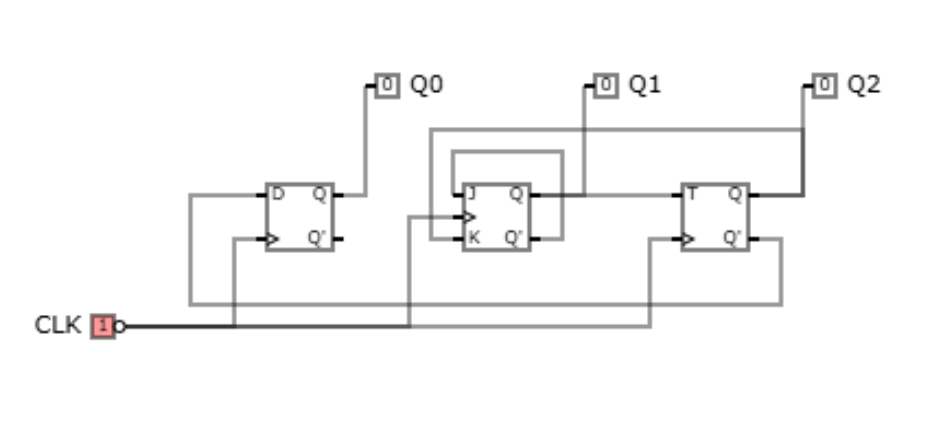
\includegraphics[scale=0.6]{Schema1.png}
\end{minipage}

\end{document}